\subsection{Part 3}
\begin{frame}
    \frametitle{Outline}
    \tableofcontents[currentsection]
\end{frame}

\begin{frame}
    \frametitle{Stability theorem proof, part 3}

    We want to prove that there exist $C_1 \geq 0, \ C_2 \geq 0$ such that
    \begin{align*}
        \| \phi(k-\drm) \| \leq C_1 + C_2 \max_{j \in \{0,\ldots,k\}} |\epsilon(j)|
    \end{align*}
    \paused
    
    We have the relationships
    \begin{align*}
        y(k) & = \frac{ q^{-\drm} B(q^{-1}) }{ A(q^{-1}) } u(k) = \frac{ B(q^{-1}) }{ A(q^{-1}) } u(k-\drm) \\
        \eta(k) & = A_c^{'}(q^{-1}) y(k) \\
        \epsilon(k) & = \eta(k) - \eta_d(k)
    \end{align*}
    which define $\epsilon(k)$ from $u(k)$ and $\eta_d(k)$.
    \pause
    
    We now invert these relationships, i.e.\ we reconstruct $u(k)$ from $\epsilon(k)$ and $\eta_d(k)$
\end{frame}

\begin{frame}
    \frametitle{Stability theorem proof, part 3}
        
    The inverted relationships are
    \begin{align*}
        u(k-\drm) & = \frac{ A(q^{-1}) }{ B(q^{-1}) } y(k) \\
        y(k) & = \frac{1}{ A_c^{'}(q^{-1}) } \eta(k) \\
        \eta(k) & = \epsilon(k) + \eta_d(k)
    \end{align*}
    \paused

    These relationships are shown in the block diagram
    \begin{figure}
        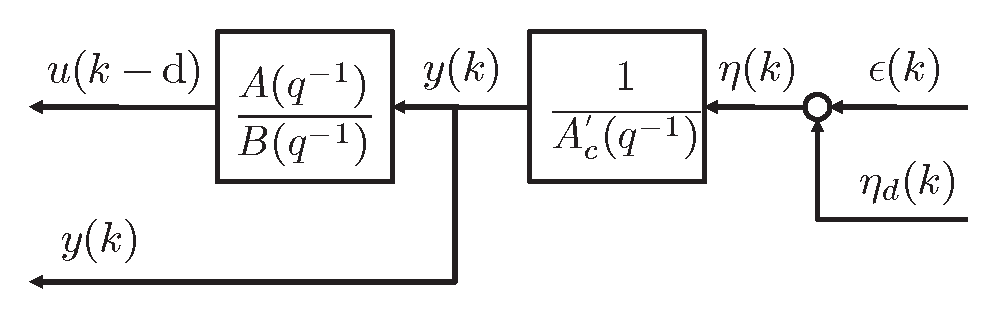
\includegraphics[width=8cm]{figs_bounded}\\
    \end{figure}
    
\end{frame}

\begin{frame}
    \frametitle{Stability theorem proof, part 3}

    \begin{figure}
        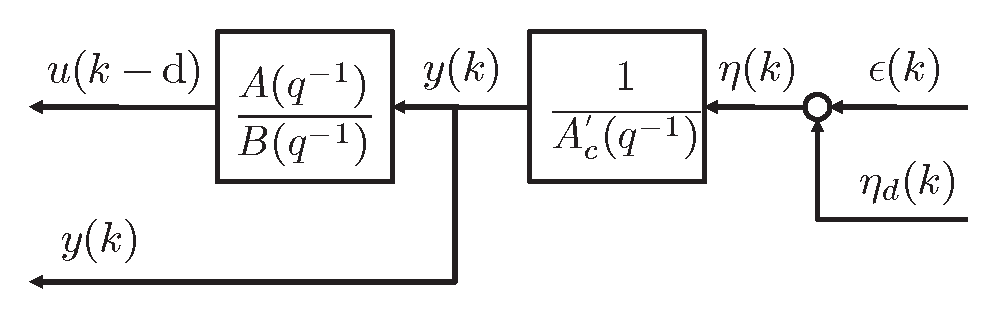
\includegraphics[width=8cm]{figs_bounded}\\
    \end{figure}
    \hrule{\hfill}
    
    Since $A_c^{'}(q^{-1})$ and $B(q^{-1})$ are anti-Schur, both blocks in the block diagram are causal and BIBO
    \pause
    
    Therefore, we can choose nonnegative $\bar{C}_{1u}$, $C_{2u}$, $\bar{C}_{1y}$, and $C_{2y}$ such that
    \begin{align*}
        |u(k-\drm)| & \leq \bar{C}_{1u} + C_{2u} \max_{j \leq k} |\eta(j)| \\
        |y(k)| & \leq \bar{C}_{1y} + C_{2y} \max_{j \leq k} |\eta(j)|
    \end{align*}

\end{frame}

\begin{frame}
    \frametitle{Stability theorem proof, part 3}

    \begin{align*}
        |u(k-\drm)| & \leq \bar{C}_{1u} + C_{2u} \max_{j \leq k} |\eta(j)| \\
        |y(k)| & \leq \bar{C}_{1y} + C_{2y} \max_{j \leq k} |\eta(j)|
    \end{align*}
    \hrule{\hfill}
    
    Assuming that $|\eta_d(k)| \leq \bar{\eta}_d$, the triangle inequality tells us that 
    \begin{align*}
        |\eta(j)| \leq |\eta_d(k)| + |\epsilon(k)| \leq \bar{\eta}_d + |\epsilon(k)|
    \end{align*}
    \paused
    
    Defining $C_{1u} = \bar{C}_{1u} + C_{2u} \bar{\eta}_d$ and $C_{1y} = \bar{C}_{1y} + C_{2y} \bar{\eta}_d$ we have
    \begin{align*}
        |u(k-\drm)| & \leq C_{1u} + C_{2u} \max_{j \leq k} |\epsilon(j)| \\
        |y(k)| & \leq C_{1y} + C_{2y} \max_{j \leq k} |\epsilon(j)|
    \end{align*}

\end{frame}

\begin{frame}
    \frametitle{Stability theorem proof, part 3}

    \begin{align*}
        |u(k-\drm)| & \leq C_{1u} + C_{2u} \max_{j \leq k} |\epsilon(j)| \\
        |y(k)| & \leq C_{1y} + C_{2y} \max_{j \leq k} |\epsilon(j)|
    \end{align*}
    \hrule{\hfill}
    
    Since $\displaystyle \max_{j \leq k-\ell} |\epsilon(j)| \leq \max_{j \leq k} |\epsilon(j)|$ for $\ell \geq 0$, we have
    \begin{align*}
        |u(k-\drm-\ell)| & \leq C_{1u} + C_{2u} \max_{j \leq k} |\epsilon(j)| \\
        |y(k-\drm-\ell)| & \leq C_{1y} + C_{2y} \max_{j \leq k} |\epsilon(j)|
    \end{align*}
    for all $\ell \geq 0$

\end{frame}

\begin{frame}
    \frametitle{Stability theorem proof, part 3}

    \vspace*{-\baselineskip}
    \begin{align*}
        |u(k-\drm-\ell)| & \leq C_{1u} + C_{2u} \max_{j \leq k} |\epsilon(j)| \\
        |y(k-\drm-\ell)| & \leq C_{1y} + C_{2y} \max_{j \leq k} |\epsilon(j)|
    \end{align*}
    \hrule{\hfill}

    Using the triangle inequality, we have
    \begin{align*}
        & \| \phi(k-\drm) \| \leq \sum_{j=0}^{n_s} \left| y(k-\drm-j) \right|
            + \sum_{i=0}^{n_r} \left| u(k-\drm-i) \right| \\
        & \hspace{.5cm} \begin{aligned}
        & \leq \sum_{j=0}^{n_s} \left( C_{1y} + C_{2y} \max_{\ell \leq k} |\epsilon(\ell)| \right)
            + \sum_{i=0}^{n_r} \left( C_{1u} + C_{2u} \max_{\ell \leq k} |\epsilon(\ell)| \right)% \\
%        & \leq \left[ (n_s+1) C_{1y} + (n_r+1) C_{1u} \right] \\
%        & \quad + \left[ (n_s+1) C_{2y} + (n_r+1) C_{2u} \right] \max_{j \leq k} |\epsilon(j)|
        \end{aligned}
    \end{align*}
    \paused
    
    Therefore
    \alignbox{
        \| \phi(k-\drm) \| & \leq \left[ (n_s+1) C_{1y} + (n_r+1) C_{1u} \right] \\
        & \quad + \left[ (n_s+1) C_{2y} + (n_r+1) C_{2u} \right] \max_{j \leq k} |\epsilon(j)|
    }

\end{frame}




